\documentclass{beamer}
\usefonttheme{professionalfonts}
\usepackage{amsmath}
\usepackage[linesnumbered,ruled,vlined]{algorithm2e}
\usepackage{tabularx}
\usepackage{makecell}
\usepackage{graphicx}
\usepackage{tikz}
\usepackage[absolute,overlay]{textpos}
\usepackage{pgfpages}

\graphicspath{{assets/}}
\setbeamertemplate{navigation symbols}{}
\setbeamerfont{caption}{size=\scriptsize}

\title[RNA ML Architecture Comparison]{\textbf{On the performance of machine learning architectures for RNA structure prediction}}
\subtitle{Bachelor thesis defense}
\author{Aaron Masur}
\date{July 13, 2026}


\newcommand{\smallcap}[1]{{\scriptsize\textbf{#1}}}
\newcommand{\takehome}[1]{\vspace{0.4em}\centering\Large $\Rightarrow$ \textbf{#1}}
\newcommand{\thesispicScale}{0.04}

% -----------------------------------------------------------------------------
% Editable chapter navigation bar
% Change these titles once you have your final structure.
\newcommand{\chapterone}{Introduction to research questions}
\newcommand{\chaptertwo}{RNA basics}
\newcommand{\chapterthree}{Machine Learning Architectures}
\newcommand{\chapterfour}{Pipeline}
\newcommand{\chapterfive}{Results}

% Set the active chapter before a frame with: \setchapternav{3}
% Hide/show the bar with: \showchapterbarfalse / \showchapterbartrue
\newif\ifshowchapterbar
\showchapterbarfalse
\newcommand{\currentchapter}{0}
\newcommand{\setchapternav}[1]{\renewcommand{\currentchapter}{#1}}

\newcommand{\chaptersegment}[2]{%
  \ifnum\currentchapter=#1
    \colorbox{blue!13}{\parbox[c][0.45cm][c]{0.185\paperwidth}{\centering\tiny\bfseries #1. #2}}%
  \else
    \colorbox{black!3}{\parbox[c][0.45cm][c]{0.185\paperwidth}{\centering\tiny\color{black!36} #1. #2}}%
  \fi
}

\setbeamertemplate{footline}{%
  \ifshowchapterbar
    {\setlength{\fboxsep}{0pt}%
    \hbox to \paperwidth{%
      \chaptersegment{1}{\chapterone}%
      \chaptersegment{2}{\chaptertwo}%
      \chaptersegment{3}{\chapterthree}%
      \chaptersegment{4}{\chapterfour}%
      \chaptersegment{5}{\chapterfive}%
      \makebox[0.075\paperwidth][c]{\tiny\color{black!45}\insertframenumber/\inserttotalframenumber}%
    }}%
  \fi
}

\begin{document}

% -----------------------------------------------------------------------------
{\setbeamertemplate{background canvas}{\begin{tikzpicture}[remember picture,overlay]
    \node[anchor=center,inner sep=0pt,opacity=0.15] at (current page.center) {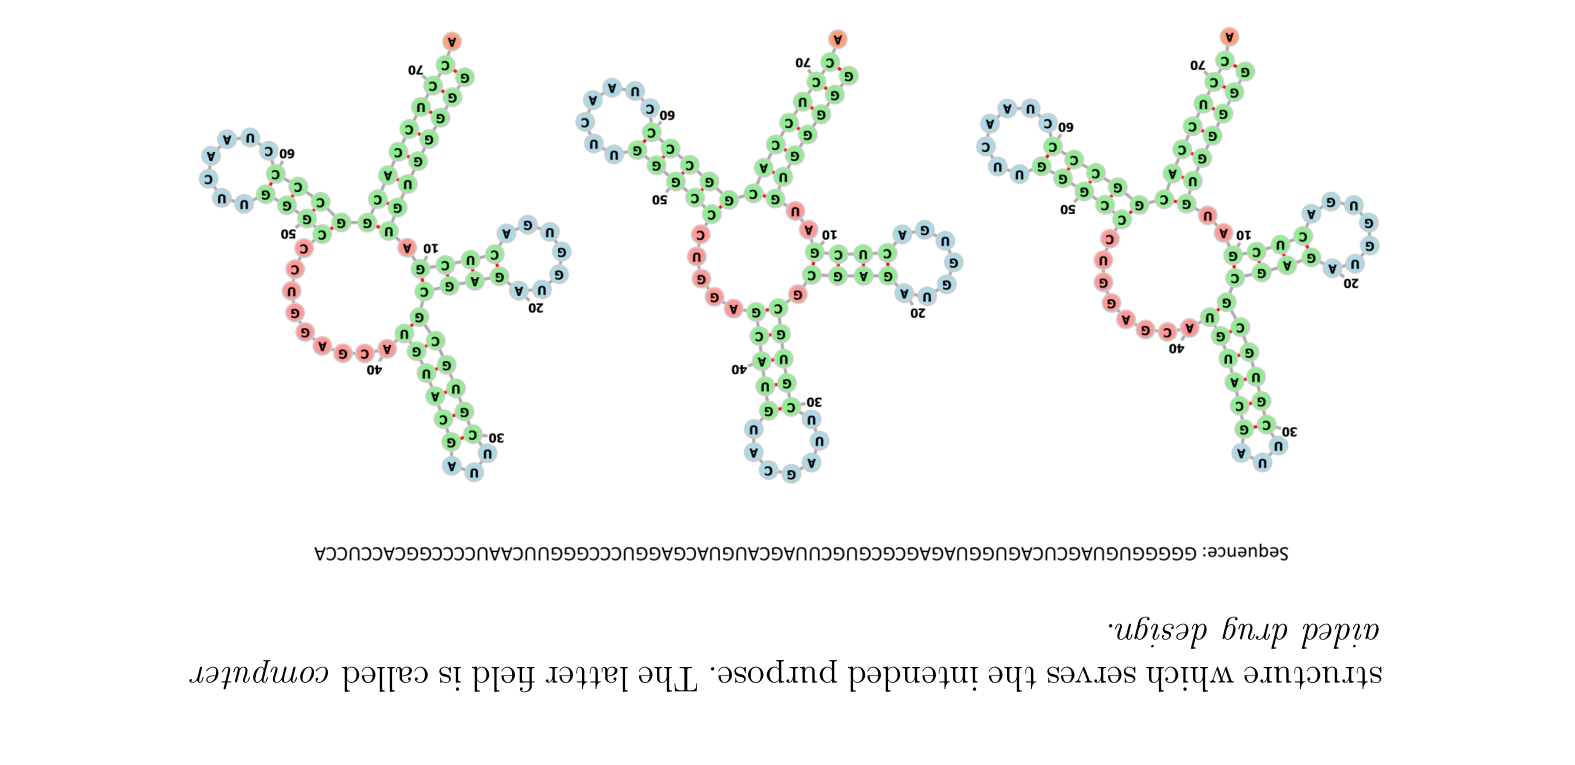
\includegraphics[width=\paperwidth,height=\paperheight,keepaspectratio]{rna_ensemble2.png}};
  \end{tikzpicture}}
\begin{frame}[plain]
  \titlepage
\end{frame}
\setbeamertemplate{background canvas}{}
}

% -----------------------------------------------------------------------------
\begin{frame}[plain]
  \begin{tikzpicture}[remember picture,overlay]
    \node[anchor=center,inner sep=0pt,opacity=1] at (current page.center) {\includegraphics[width=\paperwidth,height=\paperheight,keepaspectratio]{thesisinpictures.png}};
  \end{tikzpicture}
\end{frame}

% -----------------------------------------------------------------------------
{\setbeamertemplate{background canvas}{\begin{tikzpicture}[remember picture,overlay]
    \node[anchor=center,inner sep=0pt,opacity=0.35] at (current page.center) {\includegraphics[width=\paperwidth,height=\paperheight,keepaspectratio]{thesisinpictures.png}};
  \end{tikzpicture}}
\begin{frame}{Overview}
  \vfill
  \begin{enumerate}
    \large
    \item<1-> \chapterone
    \item<2-> \chaptertwo
    \item<3-> \chapterthree
    \item<4-> \chapterfour
    \item<5-> \chapterfive
  \end{enumerate}
  \vfill
  \note{This is intentionally only a rough map. The chapter titles are defined once in the preamble, so they can be changed later. After this slide, the same structure appears as a small navigation strip at the bottom of each slide.}
\end{frame}
\setbeamertemplate{background canvas}{}
}

\showchapterbartrue
\setchapternav{1}

% -----------------------------------------------------------------------------
\begin{frame}{The question behind the thesis}
  warum gucke ich mir das überhaupt an.
  warum ist RNA interessant?
  warum ML?
  Warum impact der modelle messen?
\end{frame}

% -----------------------------------------------------------------------------
\begin{frame}{Two research questions}
  \vfill
  \begin{enumerate}
    \item<1-> \textbf{How much data is necessary} for FFN, CNN, and BLSTM models to perform sufficiently well?
          \vspace{1em}
    \item<2-> \textbf{How do these architectures behave on biased datasets} such as base-pair span, GC content, helix length, and multiloops?
  \end{enumerate}
  \vfill
  \only<3->{\takehome{Not just ``which model wins'', but what each architecture learns.}}
  \note{Mention that RQ1 is about data scaling and the basic ability to learn RNA folding patterns. RQ2 is about stress testing: if I bias the training data in a controlled way, does the model still generalize or does it rely on that bias?}
\end{frame}

% -----------------------------------------------------------------------------
\setchapternav{2}
\begin{frame}{What is RNA?}
\end{frame}

% -----------------------------------------------------------------------------
\setchapternav{3}
\begin{frame}{The three modeling principles}
\end{frame}

% -----------------------------------------------------------------------------
\begin{frame}{FFN: fully connected, but no structural prior}
\end{frame}

% -----------------------------------------------------------------------------
\begin{frame}{CNN: local kernels on sequence and pairwise space}
\end{frame}

% -----------------------------------------------------------------------------
\begin{frame}{BLSTM: sequence context in both directions}
\end{frame}

% -----------------------------------------------------------------------------
\setchapternav{4}
\begin{frame}{Design constraints I chose deliberately}
\end{frame}

% -----------------------------------------------------------------------------
\begin{frame}{Pipeline: from data to evaluation}
  \centering
  \vspace{0.7em}
  \begin{tikzpicture}[node distance=1.3cm, >=stealth, thick]
    \tikzstyle{box}=[draw=black!65, fill=blue!5, rounded corners=4pt, minimum width=2.1cm, minimum height=0.9cm, align=center]
    \node[box] (d) {data\\generation};
    \node[box, right of=d, xshift=1.9cm] (o) {model\\optimization};
    \node[box, right of=o, xshift=1.9cm] (t) {training};
    \node[box, right of=t, xshift=1.9cm] (e) {evaluation};
    \draw[->] (d) -- (o);
    \draw[->] (o) -- (t);
    \draw[->] (t) -- (e);

    \only<1>{\draw[red, very thick, rounded corners=6pt] ([xshift=-0.18cm,yshift=-0.12cm]d.south west) rectangle ([xshift=0.18cm,yshift=0.12cm]d.north east);}
    \only<2>{\draw[red, very thick, rounded corners=6pt] ([xshift=-0.20cm,yshift=-0.12cm]o.south west) rectangle ([xshift=0.20cm,yshift=0.12cm]o.north east);}
    \only<3>{\draw[red, very thick, rounded corners=6pt] ([xshift=-0.16cm,yshift=-0.12cm]t.south west) rectangle ([xshift=0.16cm,yshift=0.12cm]t.north east);}
    \only<4>{\draw[red, very thick, rounded corners=6pt] ([xshift=-0.16cm,yshift=-0.12cm]e.south west) rectangle ([xshift=0.16cm,yshift=0.12cm]e.north east);}
  \end{tikzpicture}
  \vfill
  \begin{overlayarea}{0.85\textwidth}{4.2cm}
    \only<1>{
      \begin{minipage}{0.85\textwidth}
        \centering
        \large\textbf{Data generation}

        \vspace{0.35em}
        Synthetic RNA sequences are sampled, then labeled with RNAfold-derived secondary structures.
      \end{minipage}
    }
    \only<2>{
      \begin{minipage}{0.85\textwidth}
        \centering
        \large\textbf{Model optimization}

        \vspace{0.35em}
        Search the architecture-specific and training hyperparameters so each model gets its best setup.
      \end{minipage}
    }
    \only<3>{
      \begin{minipage}{0.85\textwidth}
        \centering
        \large\textbf{Training}

        \vspace{0.35em}
        Train with BCEWithLogitsLoss and Adam, and stop early based on validation MCC.
      \end{minipage}
    }
    \only<4>{
      \begin{minipage}{0.85\textwidth}
        \centering
        \large\textbf{Evaluation}

        \vspace{0.35em}
        Test on an independent sequence set and report MCC together with RNA-specific metrics.
      \end{minipage}
    }
  \end{overlayarea}
  \vfill
  \note{Walk through this slowly. Data generation: synthetic sequence and RNAfold label. Optimization: tune architecture and non-architecture hyperparameters such as threshold and positive class weight. Training: BCEWithLogitsLoss plus Adam, early stopping on validation MCC. Evaluation: independent test set, MCC and RNA-specific metrics.}
\end{frame}

% -----------------------------------------------------------------------------
\setchapternav{5}
\begin{frame}{RQ1 setup: how much data is enough?}
  \vfill
  \begin{center}
    \renewcommand{\arraystretch}{1.28}
    \begin{tabular}{c|c|c|c|c|c}
      \textbf{train size} & 200  & 1,000 & 5,000    & 10,000 & 50,000  \\
      \hline
      \textbf{idea}       & tiny & small & moderate & large  & scaling
    \end{tabular}
  \end{center}
  \vspace{1em}
  \large
  Each optimized architecture is trained on each size and evaluated on an independent 10,000-sequence test set.\\[0.6em]
  Primary score: \textbf{MCC}. Additional RNA metrics: symmetry, sparsity, non-canonical ratio, minimum loop length.
  \note{Mention that MCC is useful because base-pair matrices are very imbalanced: almost all cells are zeros. Accuracy would be misleading. The extra RNA metrics explain what the model learned structurally, not just whether the MCC went up.}
\end{frame}

% -----------------------------------------------------------------------------
\begin{frame}{RQ1 result: MCC scaling}
  \centering
  \renewcommand{\arraystretch}{1.25}
  \begin{tabular}{c|ccccc}
    \textbf{Model} & \textbf{200} & \textbf{1,000} & \textbf{5,000} & \textbf{10,000} & \textbf{50,000} \\
    \hline
    FFN            & 0.0104       & 0.0184         & 0.0257         & 0.0272          & 0.0280          \\
    CNN            & 0.2711       & 0.3165         & 0.3997         & 0.3976          & 0.4260          \\
    BLSTM          & 0.0000       & 0.0000         & 0.2924         & 0.3043          & 0.3359          \\
  \end{tabular}
  \vfill
  \only<2->{\takehome{CNN works early; BLSTM needs roughly 5,000; FFN stays near zero.}}
  \note{This is one of the central slides. Say: FFN is basically not solving the task. CNN already gets a meaningful MCC at 200 and improves with data. BLSTM is flat at zero for 200 and 1000 because predictions are below its optimized threshold; after 5000 it starts producing meaningful structures.}
\end{frame}

% -----------------------------------------------------------------------------
\begin{frame}{RQ1 visual result: what the models predict}
  \centering
  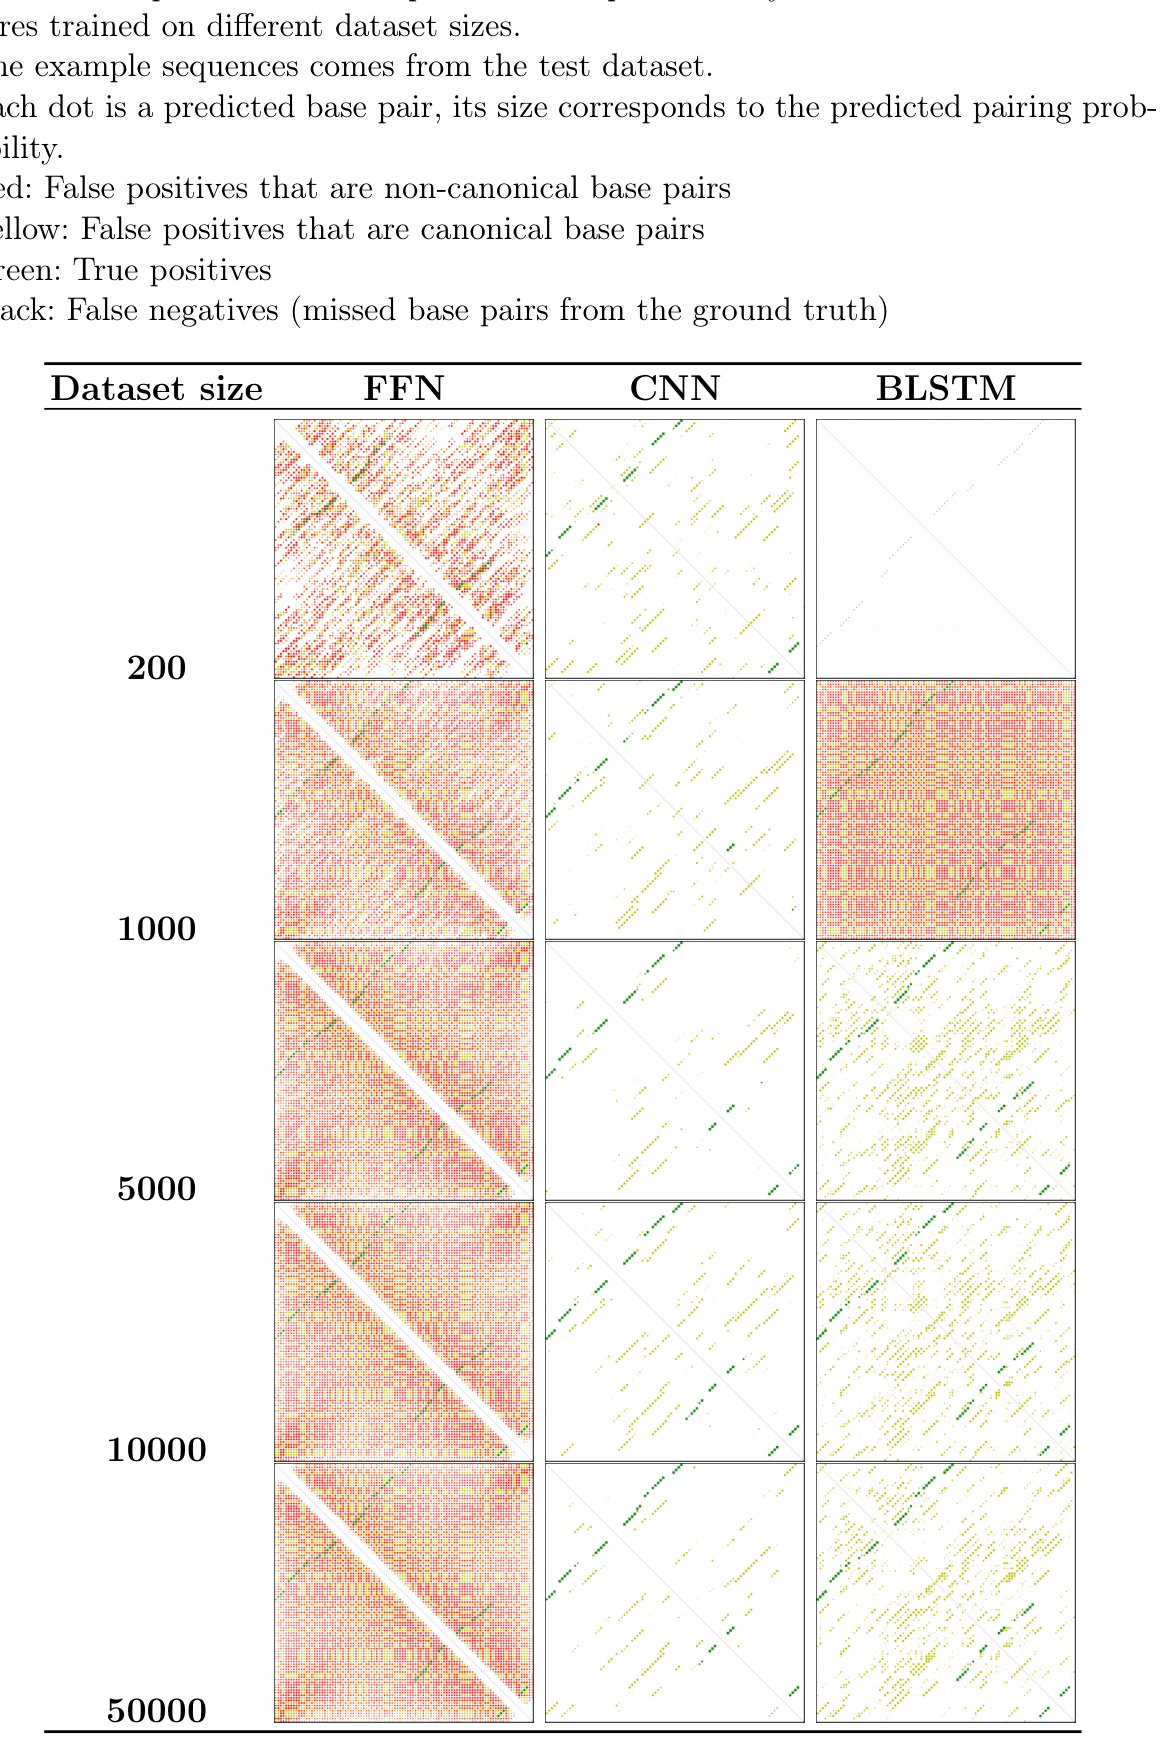
\includegraphics[width=0.82\textwidth,height=0.73\textheight,keepaspectratio]{rq1_bpm_table.png}
  \note{Use the picture more than the numbers. FFN forms a broad average-looking pattern with many false positives, rather than sequence-specific folding. CNN predictions are sparse and already close to real base-pair diagonals. BLSTM with little data is too diffuse or below threshold, then begins to show structure from 5000 onward.}
\end{frame}

% -----------------------------------------------------------------------------
\begin{frame}{RQ1 RNA metrics: low vs. high data}
  \vfill
  \begin{minipage}{0.49\textwidth}
    \centering
    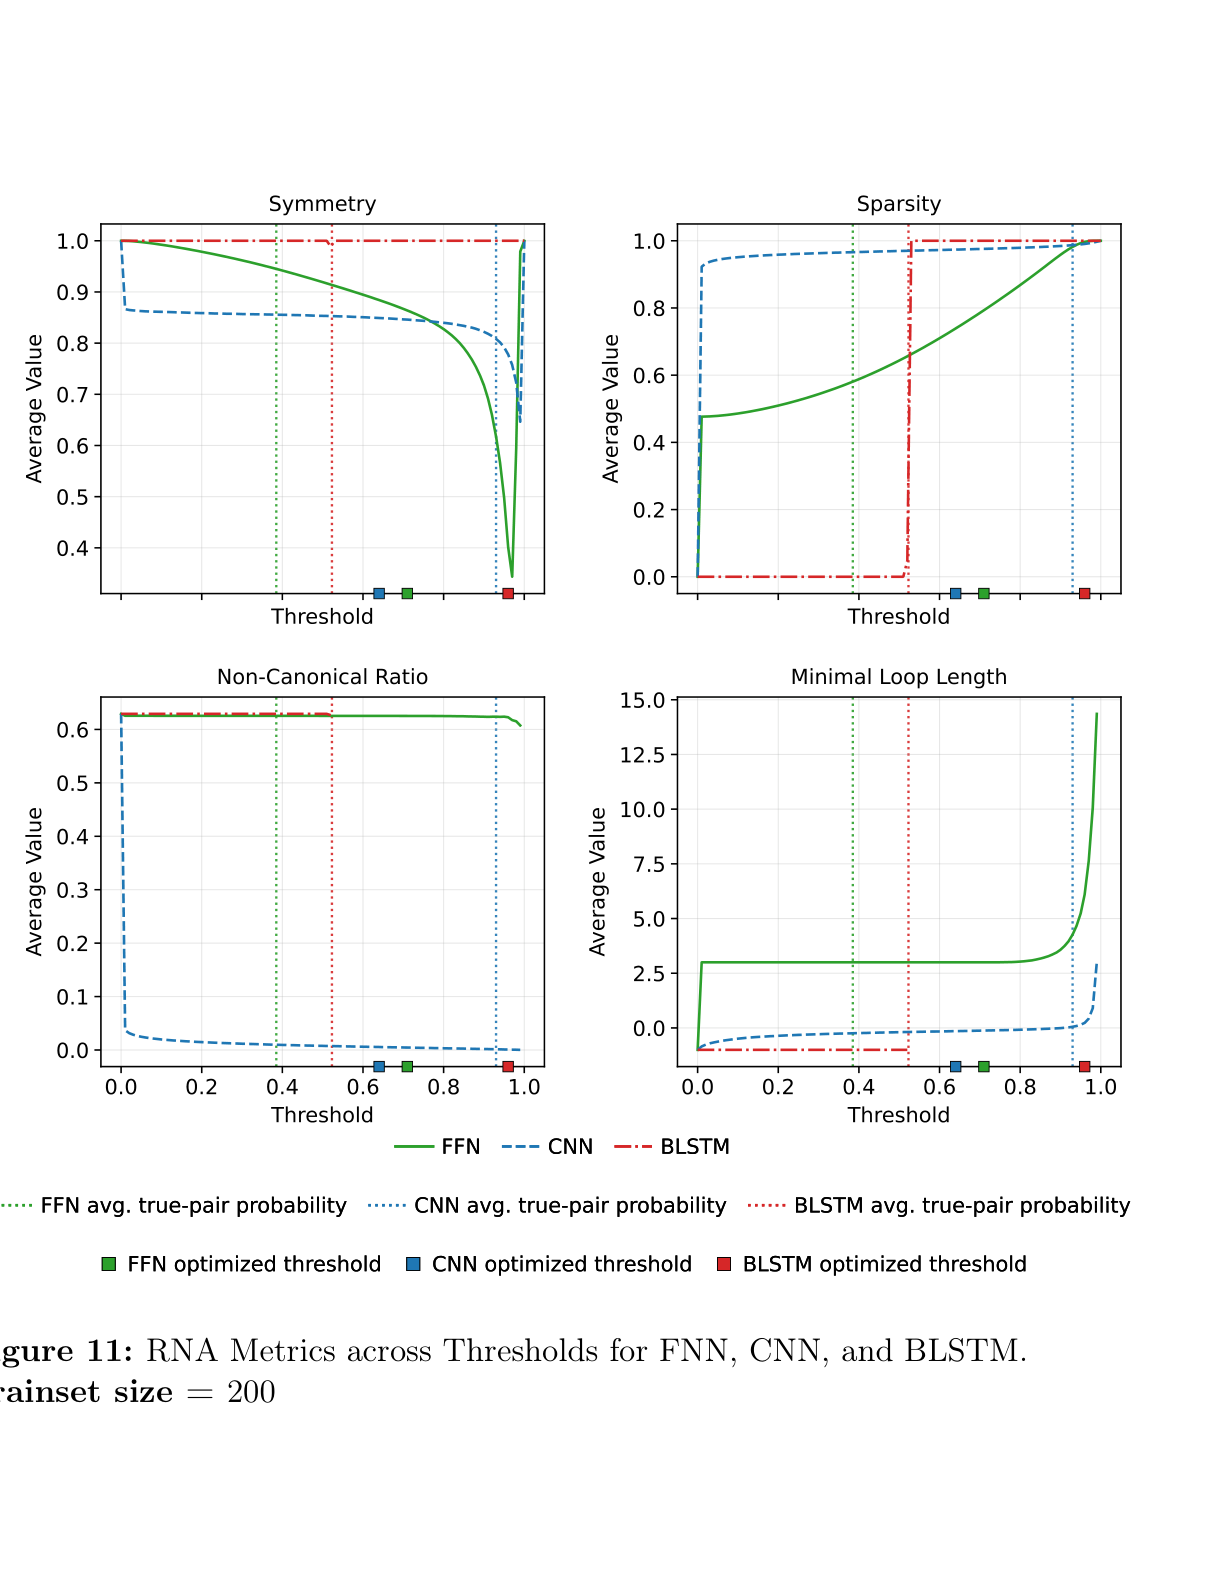
\includegraphics[width=\linewidth,keepaspectratio]{rq1_metrics_200.png}\\[3pt]
    \footnotesize train size 200
  \end{minipage}\hfill
  \begin{minipage}{0.49\textwidth}
    \centering
    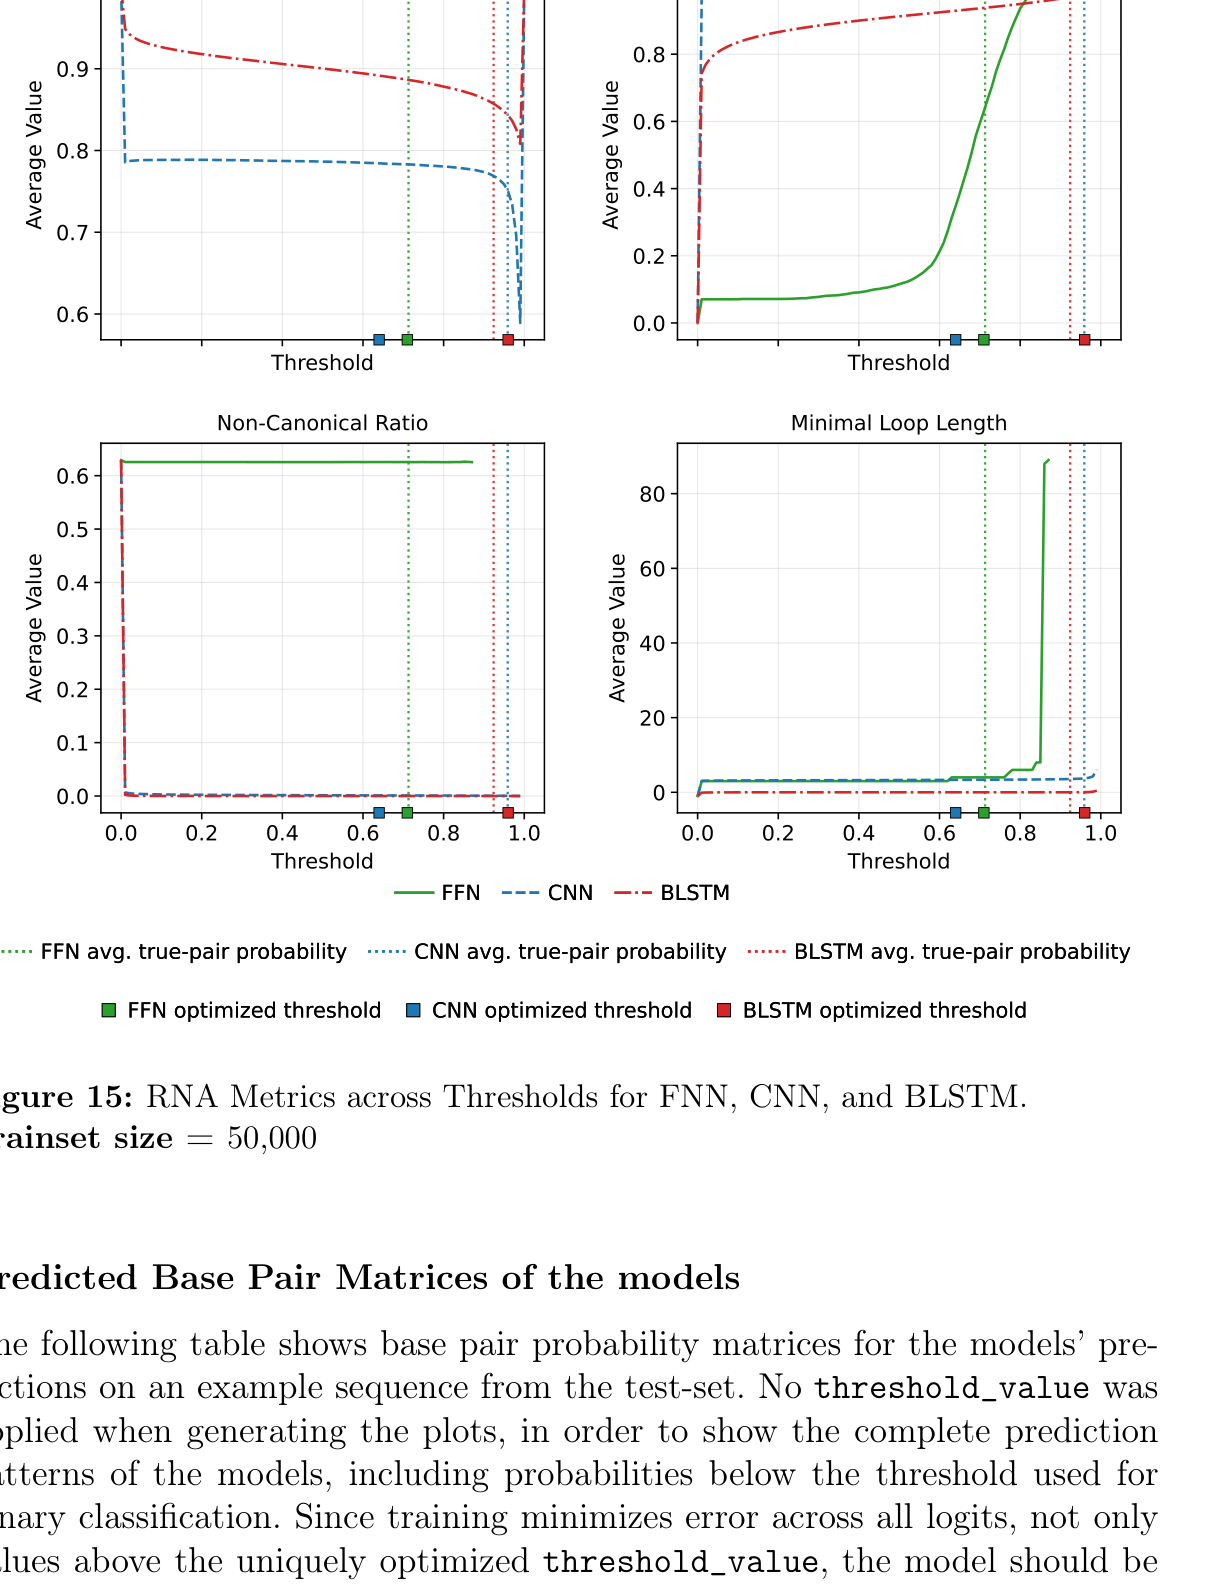
\includegraphics[width=\linewidth,keepaspectratio]{rq1_metrics_50000.png}\\[3pt]
    \footnotesize train size 50,000
  \end{minipage}
  \vfill
  \note{The exact curves are not something the audience must memorize. Main story: CNN learns RNA constraints surprisingly early, but overfits. BLSTM becomes useful only with more data and still does not learn minimum loop length. FFN's curves reflect a learned average matrix rather than RNA-specific folding.}
\end{frame}

% -----------------------------------------------------------------------------
\begin{frame}{RQ1 interpretation by architecture}
  \vfill
  \begin{tabularx}{\textwidth}{@{}>{\bfseries}l X@{}}
    FFN   & learned an average base-pair distribution, not a sequence-specific folding rule                   \\[0.9em]
    CNN   & strong with little data, good local constraints, but clear overfitting                            \\[0.9em]
    BLSTM & no useful thresholded predictions for 200/1,000; starts around 5,000; weak on minimum loop length \\
  \end{tabularx}
  \vfill
  \takehome{Architecture bias explains a lot of the behavior.}
  \note{This slide maps observations to the architectural hypotheses: FFN has no locality or sequence prior. CNN has local kernels, so it is strong on local motifs and constraints. BLSTM has sequence context and lower parameter count, so it generalizes differently, but it is not naturally forced to respect local matrix constraints.}
\end{frame}

% -----------------------------------------------------------------------------
\begin{frame}{RQ2 setup: biased datasets}
  \begin{minipage}{0.43\textwidth}
    \centering
    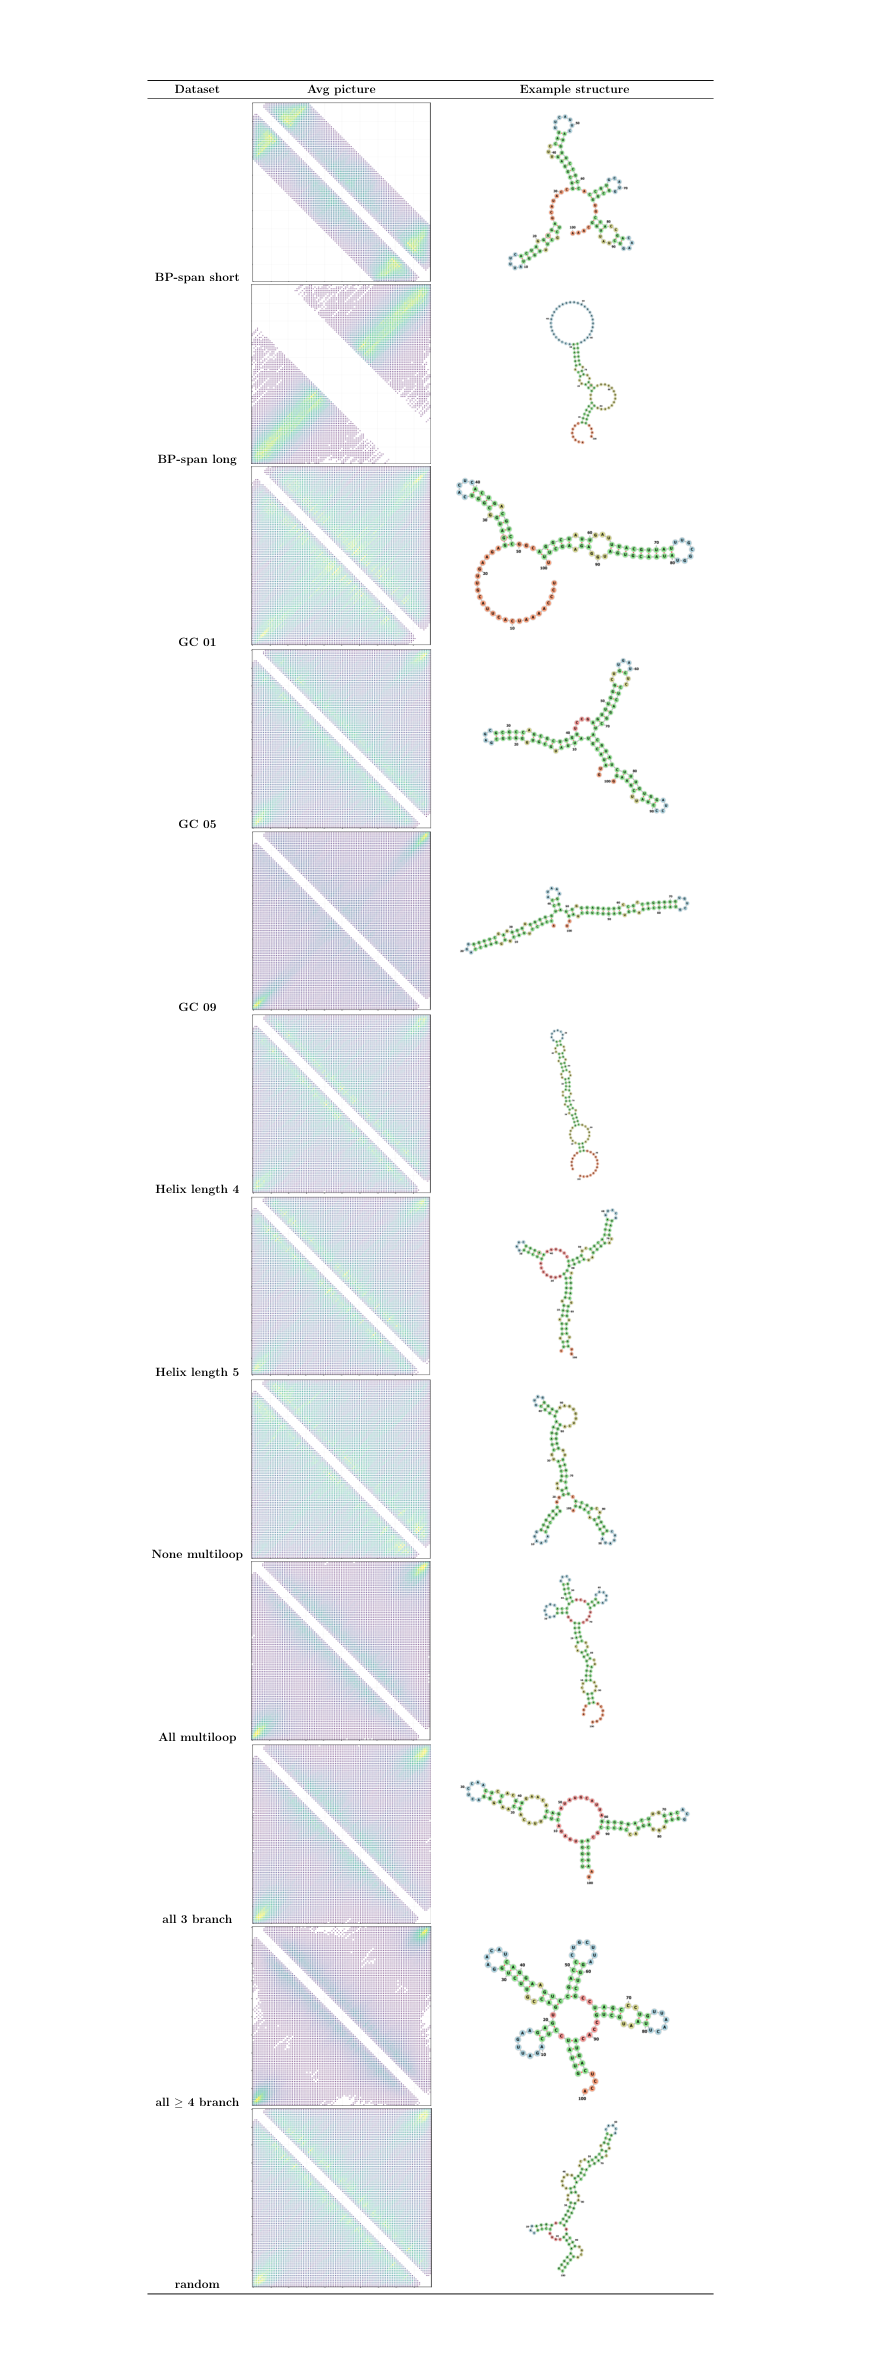
\includegraphics[height=0.78\textheight,keepaspectratio]{rq2_avg_structures.png}
  \end{minipage}\hfill
  \begin{minipage}{0.53\textwidth}
    \large
    Models were trained and evaluated across controlled biases:\\[0.7em]
    \begin{itemize}
      \item base-pair span
      \item GC content
      \item helix length
      \item multiloop topology
    \end{itemize}
  \end{minipage}
  \note{Explain that RQ2 is a transfer setup. Train on one biased dataset, evaluate on all datasets in the same experiment. This makes it possible to see whether a model learned a general rule or mostly adapted to the training distribution.}
\end{frame}

% -----------------------------------------------------------------------------
\begin{frame}{RQ2: base-pair span and GC content}
  \centering
  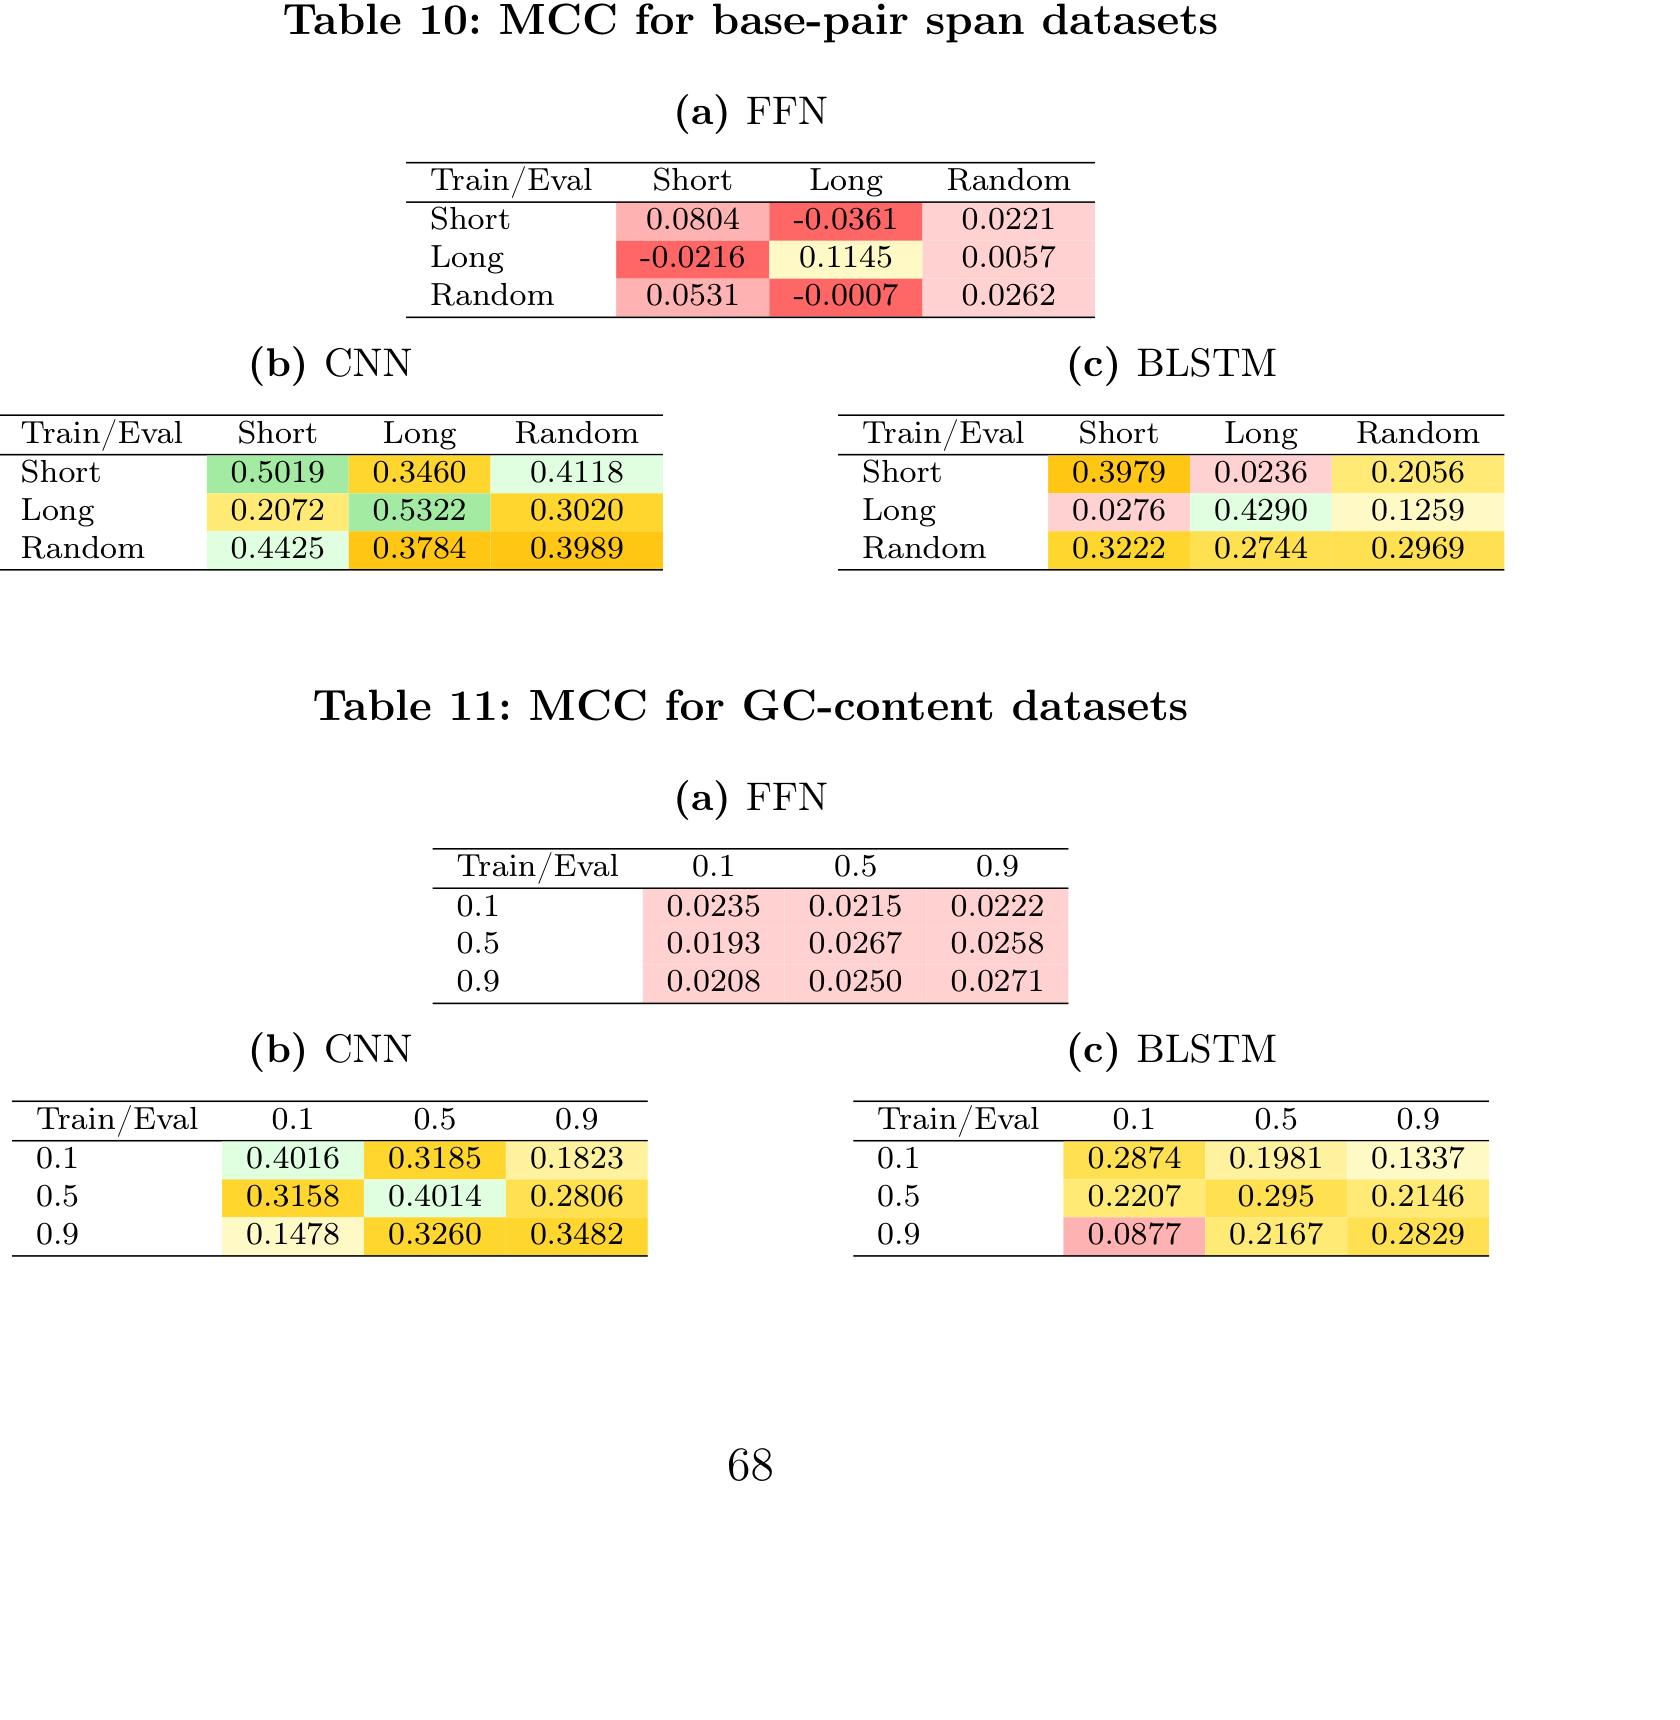
\includegraphics[width=0.88\textwidth,height=0.76\textheight,keepaspectratio]{rq2_bp_gc_tables.png}
  \note{Talk through patterns, not every number. Base-pair span: CNN and BLSTM both suffer when train and eval span distributions differ, but BLSTM is especially sensitive to span shifts. GC content: performance drops towards extreme mismatches, especially for BLSTM. FFN remains low and mainly reflects average matrix similarity.}
\end{frame}

% -----------------------------------------------------------------------------
\begin{frame}{RQ2: helix length and multiloops}
  \centering
  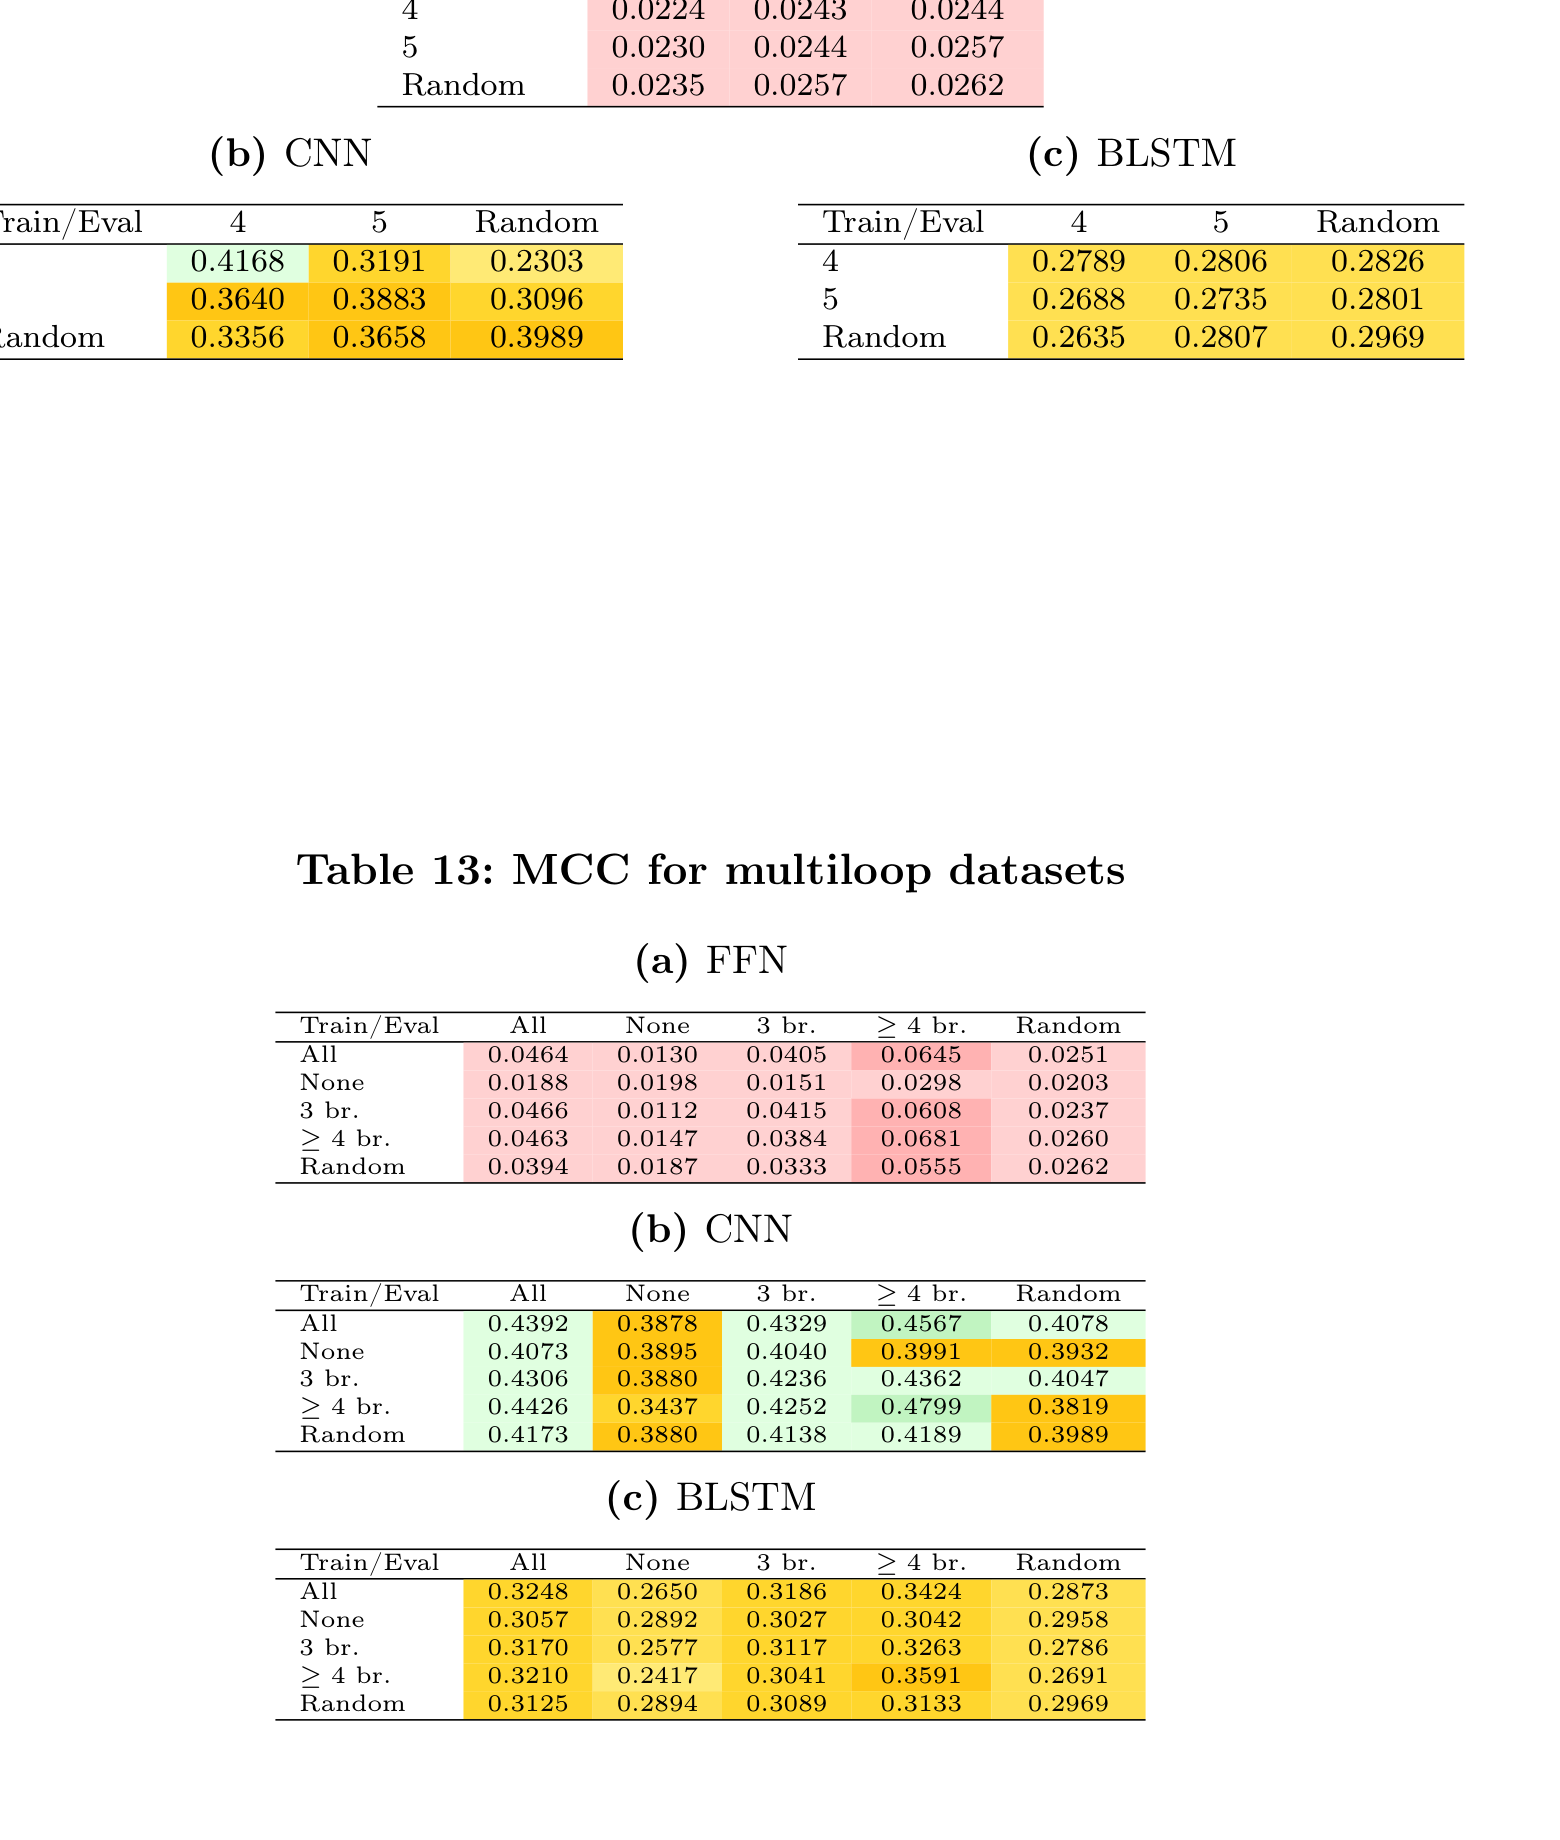
\includegraphics[width=0.86\textwidth,height=0.76\textheight,keepaspectratio]{rq2_hl_multi_tables.png}
  \note{Helix length is where the CNN sensitivity is most visible. The hypothesis is that kernels learn local helix motifs; if the helix-length distribution shifts, those patterns transfer less well. Multiloop shifts look less dramatic in MCC. Important caveat: MCC compares base-pair matrix cells and may not be a good metric for higher-order topology such as multiloop branch structure.}
\end{frame}

% -----------------------------------------------------------------------------
\begin{frame}{RQ2 interpretation}
  \vfill
  \begin{tabularx}{\textwidth}{@{}>{\bfseries}l X@{}}
    FFN        & mostly follows the average picture of train vs. evaluation set           \\[0.9em]
    BLSTM      & more sensitive to base-pair span and GC-content shifts                   \\[0.9em]
    CNN        & more sensitive to helix-length bias, likely due to kernel-learned motifs \\[0.9em]
    Multiloops & differences are moderate; MCC may hide topology errors                   \\
  \end{tabularx}
  \vfill
  \note{This slide should sound like the conclusion of RQ2. The sensitivities are not random; they can be explained from the architecture. FFN averages, CNN kernels, BLSTM sequential propagation. For multiloops, the result is also a metric lesson.}
\end{frame}

% -----------------------------------------------------------------------------
\begin{frame}{Overall take-home}
  \vfill
  \Large
  Plain architectures alone do \textbf{not} reach engineered RNA folding tools.\\[0.9em]
  But they reveal characteristic strengths and failure modes.\\[1.1em]
  \begin{center}
    \begin{tabular}{c|c}
      \textbf{Architecture} & \textbf{main lesson}            \\
      \hline
      FFN                   & learns dataset average          \\
      CNN                   & good local motifs, overfits     \\
      BLSTM                 & needs more data, global context \\
    \end{tabular}
  \end{center}
  \vfill
  \note{Connect back to the motivation: high performance of modern tools probably depends substantially on constraints, postprocessing, and specialized/hybrid designs. Architecture matters, but architecture alone is not enough here.}
\end{frame}

% -----------------------------------------------------------------------------
\begin{frame}{Outlook}
  \vfill
  \begin{minipage}{0.48\textwidth}
    \large
    \begin{itemize}
      \item hybrid architectures
      \item equal parameter-count comparison
      \item multiple random seeds
      \item finer bias sweeps
    \end{itemize}
  \end{minipage}\hfill
  \begin{minipage}{0.48\textwidth}
    \large
    \begin{itemize}
      \item real biological RNA datasets
      \item variable-length sequences
      \item transformers / graph neural networks
      \item topology-aware multiloop metrics
    \end{itemize}
  \end{minipage}
  \vfill
  \note{This is where you can say what you would do with more time. Especially emphasize hybrid architectures, because the results suggest complementary strengths. Also equal model complexity is important because the CNN had many more parameters than the BLSTM.}
\end{frame}

% -----------------------------------------------------------------------------
\begin{frame}{Danke für die Aufmerksamkeit!}
  \begin{center}
    \vfill
    \Huge Questions?
    \vfill
    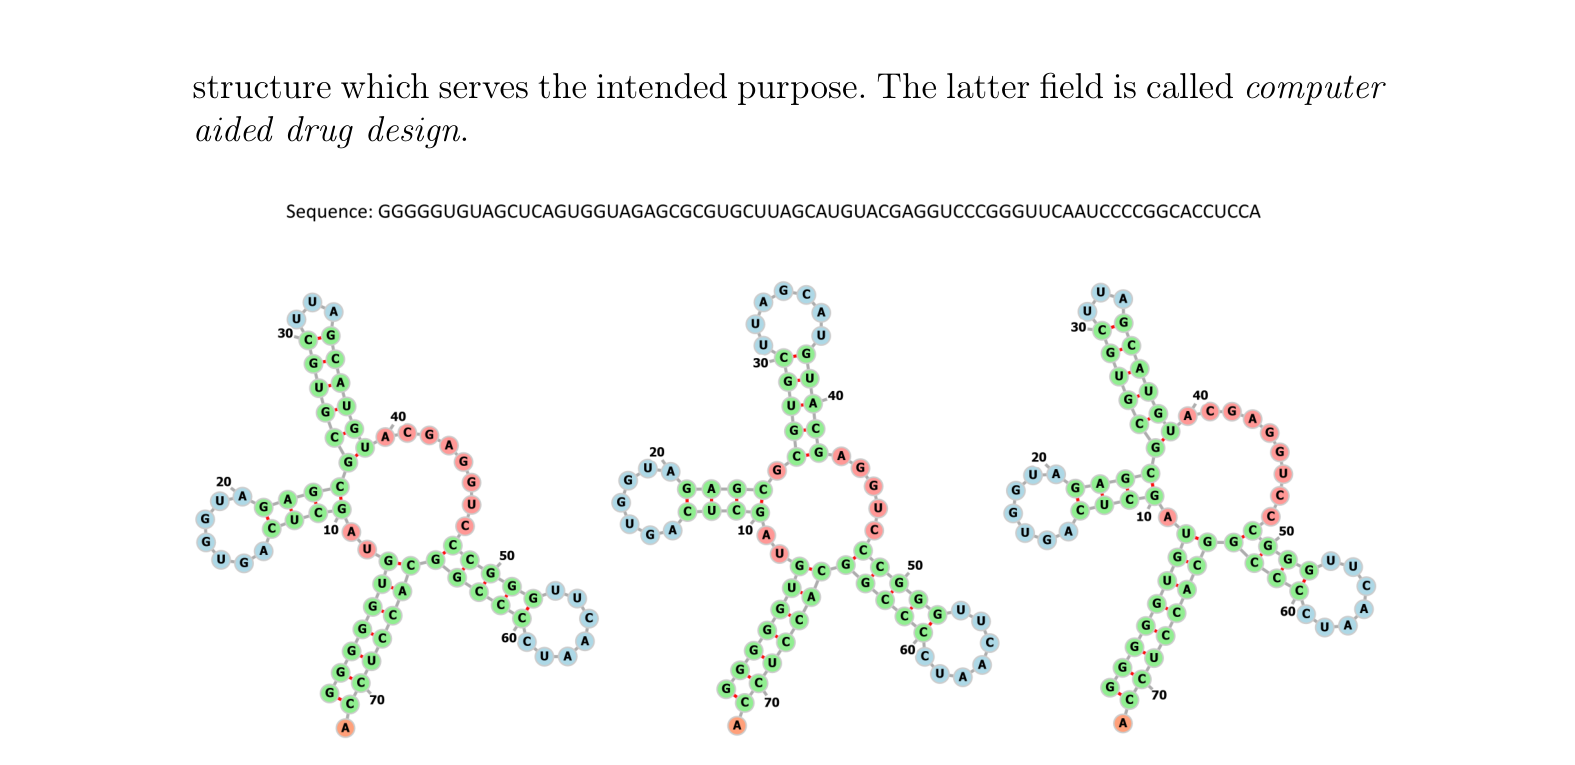
\includegraphics[width=0.64\textwidth,keepaspectratio]{rna_ensemble.png}
    \vfill
  \end{center}
  \note{End relaxed. If asked about limitations, answer honestly: synthetic labels, fixed length, no regularization, limited architectures, and MCC limitations. Then explain why each was chosen.}
\end{frame}

\end{document}
